%! Author = vova
%! Date = 03.10.2020

% Preamble
\documentclass[11pt]{memoir}

% Packages
\usepackage{amsmath}
\usepackage{romannum}
\usepackage{hyperref}
\usepackage{graphicx}
\usepackage{setspace}
\usepackage{tikz}
\usepackage{import}
% \usepackage{pygmentize}
% \usepackage{minted}

\usetikzlibrary{circuits}
\usetikzlibrary{circuits.ee}
\usetikzlibrary{circuits.ee.IEC}
\usetikzlibrary{circuits.logic.IEC}


\title{\textbf{\Huge{Measuring resistance using non-ideal devices}}}
\date{03.10.2020}
\author{Latipov Vladimir \&\& Onishenko Sergiy}


% Document
\begin{document}
    \maxtocdepth{subsection}
    % \setsecnumdepth{subsection}
    \renewcommand{\thesection}{\arabic{section}}
    \pagenumbering{gobble}
    % \thispagestyle{empty}

    \maketitle
    \newpage
    \pagenumbering{arabic}

    \tableofcontents

    \newpage


    \begin{vplace}
    \begin{center}

    \section{Abstract}\label{sec:abstract}
            It tends to be pretty difficult and obviously not convenient to perform measurements using voltage and current sensors whose impedance is comparable with the impedance of resistor itself.\newline
            That's why it makes sense to apply optimization methods to improve accuracy.\newline
            So, we've constructed all the possible schemes and proved, that there aren't any other reasonable schemes can be constructed using the given set of instruments.\newline
            Finally, we've extracted all the data from those schemes.\newline

    \end{center}
    \end{vplace}

    \newpage

    \section{The Plan}\label{sec:the-plan}
        The task is to measure the impedance of the given resistor as precise as possible.\newline
        To achieve this aim, we decided to perform these operations:\newline

        \begin{itemize}
            \item Compute the resistance and its dispersion individually for each scheme
            \item Deduct which scheme's results stand out from the center ($\mu$), for example, the threshold value of remoteness from the center might be equal to $2 \cdot \sigma$
            \item Dropout the data outliers (outstanding measurements)
            \item For those verified measurements we use them to construct an equation system.
            \item Optimize the function which is ${\sum_{i=0}^{i<n_{equations}} \left(EQ_{i_{left}} - EQ_{i_{right}}\right) ^ 2}$\newline
                where $EQ_{i_{left}}$ and $EQ_{i_{right}}$ are left and right sides of $i^{th}$ equation respectively
            \item \label{itm:low-dispersion} As the result, we'll find the resultant resistance.\newline
            Obviously, the target function won't be equal to zero because we have 8 equations and only one variable, but the accuracy of the result will be significantly better than it is for all the initial results.
            \item Thus, the final result should be definitely found this way.
        \end{itemize}

    \section{Schemes and Equations}\label{sec:schemes-and-equations}
        There are only 8 \textit{\textbf{reasonable}} schemes can be assembled using these items:
        \begin{itemize}
            \item Exactly one battery
            \item Exactly one resistor to measure
            \item Not more than one amperemeter
            \item Not more than one voltmeter
        \end{itemize}

        Here are the schemes:

    % Scheme 1
    \subsection{Scheme 1}\label{subsec:scheme-1}

            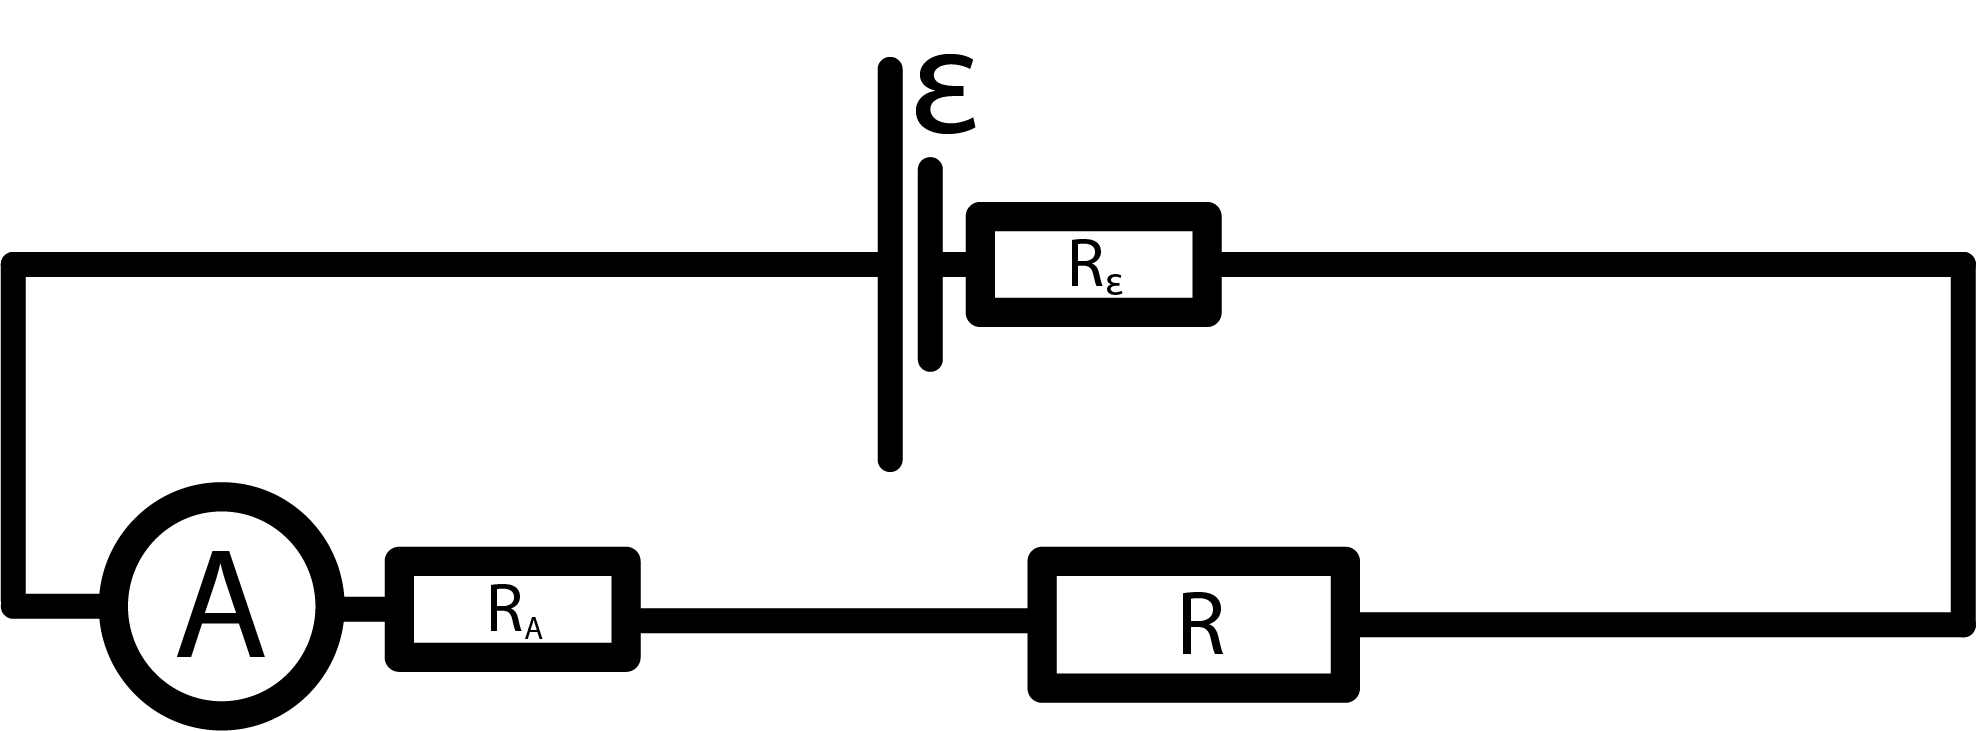
\includegraphics[width=\linewidth]{../schemes/Scheme1.png}

            \begin{equation*}
                A = \frac{\varepsilon}{R_\varepsilon + R_A + R}
            \end{equation*}

            \begin{equation}\label{eq:equation1}
                R = \frac{\varepsilon}{A_1} - R_\varepsilon - R_A
            \end{equation}

    \newpage

    % Scheme 2:
    \subsection{Scheme 2}\label{subsec:scheme-2}

    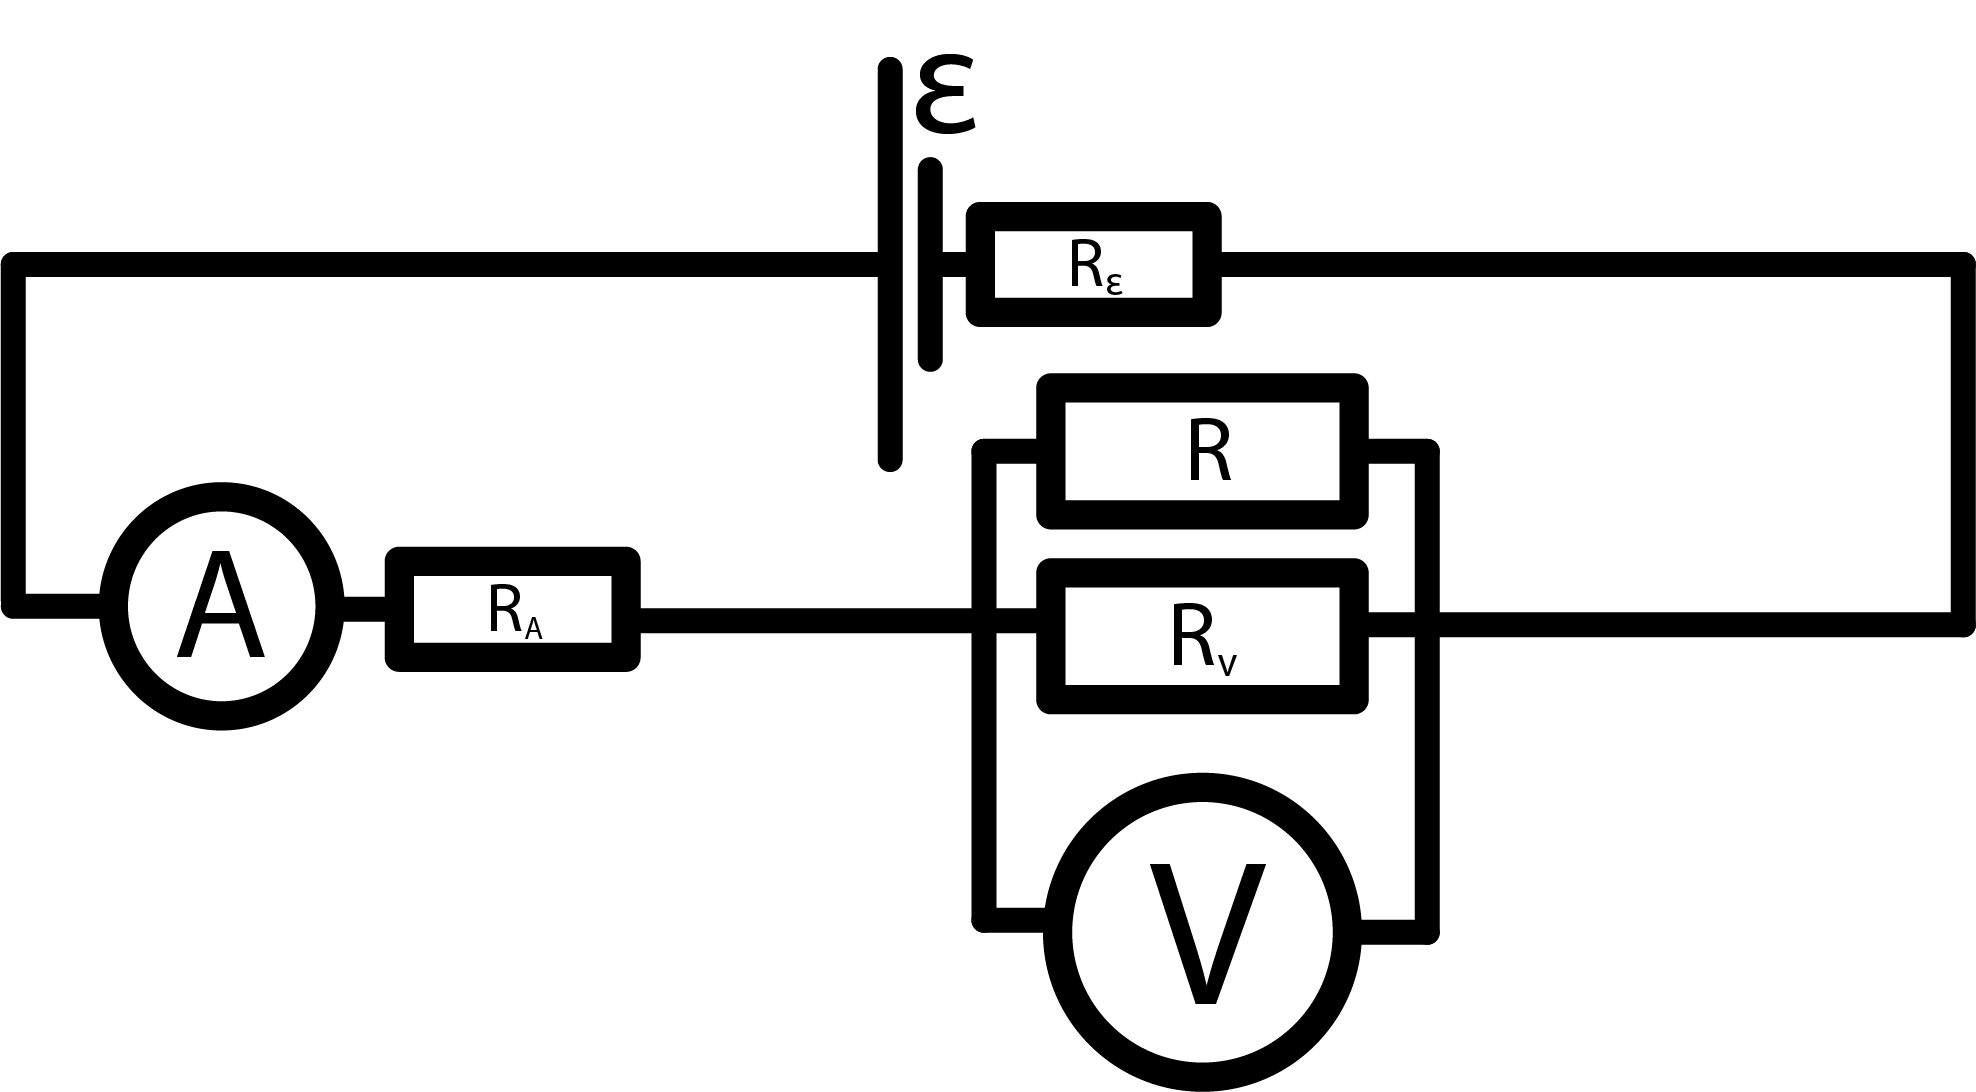
\includegraphics[width=\linewidth]{../schemes/Scheme2.png}

    \begin{equation*}
        A = \frac{\varepsilon}{R_\varepsilon + R_A + \frac{1}{\frac{1}{R} + \frac{1}{R_V}}}
    \end{equation*}

    \begin{equation}\label{eq:equation2}
    R = \frac{\varepsilon}{A_1} - R_\varepsilon - R_A
    \end{equation}


%
%        \begin{minted}[linenos]{c}
%            inline void some_func() {
%                printf("Hello, world!");
%            }
%        \end{minted}
%

    \section {Dispersion}\label{sec:dispersion}
        We've tried to perform the measurements more than once, but soon I realized, that it's quite a stupid idea. The random dispersion is negligibly small compared to the measurement dispersion.\newline
        As mentioned above (\nameref{itm:low-dispersion}), the accuracy of the result will be significantly better than it is for all the initial results.

    \section{Measurement Results}\label{sec:measurement-results}

    \section {Looking for Data Outliers}\label{sec:looking-for-data-outliers}

    \section{Optimizing the Target Function}\label{sec:optimizing-the-target-function}


    \section{The Answer}\label{sec:answer}


    \section{Conclusion}\label{sec:conclusion}



%    \begin{figure}[h!]
%        \begin{center}
%            \begin{circuitikz}
%                \draw (0,0)
%                to[V=$U_q$] (0,2) % The voltage source
%                to[short] (2,2)
%                to[R=$R_1$] (2,0) % The resistor
%                to[short] (0,0);
%            \end{circuitikz}
%            \caption{My first circuit.}
%        \end{center}
%    \end{figure}

\end{document}